% ============================================================================
% Appendix B: a neural-network model of the density, as an independent model
% of the same quantity as appendix A. To be \input after appendix A.
% Figures: fig_B_*.pdf (docs/paper/figs_appendices.py, merged_test.py).
% ============================================================================
\section{A neural-network model of the density}
\label{app:B}

To test whether the results of appendix~\ref{app:A} depend on the choice of splines and prior, we built a second
model of the same 23 coefficient functions in an entirely different way, as a neural network. It uses the same
form~(\ref{eq:A:form}), the same data, the same measures of accuracy and calibration, and, like the smooth model,
it is compared with POWHEG through bin integrals. This appendix describes only what differs.

\subsection{The network}
\label{app:B:network}

The 23 coefficient functions are densities in $m_{hh}$, given by
\begin{equation}
  a_i(m) = \phi(m)\,P_i(z)\,e^{Q_i(z)}, \qquad z = 2\sqrt{\frac{m - 2m_h}{1455~\text{GeV} - 2m_h}} - 1 ,
  \label{eq:B:net}
\end{equation}
with the threshold factor $\phi$ of eq.~(\ref{eq:A:spline}). $P$ is a fully connected network with one input, six
hidden layers of 25 units and 23 outputs, with SiLU activations, $x/(1 + e^{-x})$~\cite{Elfwing:2018,Hendrycks:2016},
and a $\tanh$ on the outputs; $Q$ is a single linear layer. The factor $e^{Q_i}$ sets the overall size of each
function, which differs by orders of magnitude between functions, and $P_i \in (-1,1)$ its shape and sign. The
network has 3,944 parameters. Two choices matter. The input $z$, like the spline breakpoints of
appendix~\ref{app:A}, gives the region 255--435~GeV, where the functions change fastest, a third of its range; with
an input linear in $m_{hh}$ that region occupies 12\% of the range, and a network of this size does not fit it. A
smooth activation makes the density smooth, where ReLU activations would make each $a_i$ piecewise linear in $z$.

\subsection{Bin integrals by Gauss--Legendre quadrature}
\label{app:B:quadrature}

As for the smooth model, the prediction for bin $k$ is the integral of the density over the bin,
$f_k(\theta) = \sum_i C_i(\theta)A_{ik}$ with $A_{ik} = \int_{\text{bin }k}a_i\,dm$. We compute $A_{ik}$ at every
training iteration by Gauss--Legendre quadrature with $n = 8$ nodes per bin,
\begin{equation}
  A_{ik} \simeq \sum_{g=1}^{n} w_{kg}\, a_i(m_{kg}),
  \label{eq:B:gl}
\end{equation}
which is exact for polynomials of degree up to $2n - 1 = 15$. The nodes and weights are computed once, as the
eigenvalues and eigenvector components of a tridiagonal matrix~\cite{Golub:1969}. The accuracy of the quadrature
matters because the loss sees only the sums~(\ref{eq:B:gl}): a quadrature error would not appear in the fit, but as a
bias in the learned density. With eight nodes the relative error of a bin integral is below $3\times10^{-5}$, against
$8\times10^{-4}$ for the model-error coefficient $\varepsilon$ at threshold; the trapezoid rule would need a spacing of
about 1~GeV near threshold to reach $10^{-3}$. Because the $a_i$ depend on $m$ only, the network is evaluated at the
640 fixed nodes once per iteration, whatever the number of training rows in the batch, and each row only selects
row $k$ of the table $A_{ik}$.

\subsection{Training}
\label{app:B:training}

The network is trained on the bins used for fitting in appendix~\ref{app:A:data}, apart from a small validation set, in two
stages, each a fixed number of iterations of the Adam optimiser~\cite{Kingma:2014vow}.
\begin{enumerate}
  \item The absolute difference $|t - f|$, averaged over mini-batches of 2,048 rows, for 200,000 iterations, with a
    learning rate of $2\times10^{-3}$ halved every 50,000 iterations.
  \item The Huber function~\cite{Huber:1964} (with threshold 2) of the pulls $(f - t)/s$, averaged over all training
    rows, for 5,000 iterations, with a learning rate of $10^{-4}$ halved every 1,250 iterations. The variance $s^2$ is
    the Poisson variance of the network's own prediction, held fixed within each iteration, so that, as in
    appendix~\ref{app:A:fit}, the fit is not biased low. The parameters with the lowest loss on a small validation set
    are kept.
\end{enumerate}
In the second stage a smoothness penalty $\lambda R$ is added to the loss, with
\begin{equation}
  R = \frac{1}{23}\sum_{i=1}^{23}\frac{\sum_j \big(g_i''(z_j)\big)^2}{\sum_j g_i(z_j)^2}, \qquad g_i = P_i\,e^{Q_i},
  \label{eq:B:penalty}
\end{equation}
the relative curvature of the network's part of each function (without the threshold factor), evaluated by second
differences on 1,201 equally spaced values of $z$, the variable in which the splines of appendix~\ref{app:A} are
uniformly spaced. The data constrain the poorly determined functions $a_{16}$--$a_{19}$ weakly, and without the penalty the
network fills that freedom with small-scale oscillations: their curvature was 10 to 300 times that of the smooth model's.
With $\lambda = 10^{-6}$ it falls to the level of the smooth model's, the curvature of $a_1$--$a_{15}$ is unchanged, and the
accuracy improves slightly; larger values make the network smoother than the smooth model and, at $\lambda = 10^{-4}$, less
accurate.

\subsection{Results}
\label{app:B:results}

\begin{table}[!htbp]
\centering
\small
\begin{tabular}{lccc}
\toprule
 & \multicolumn{2}{c}{mean $-2\ln\lambda$ per bin} & median \\
 & 255--555 GeV & $>555$ GeV & per spectrum \\
\midrule
smooth model (appendix~\ref{app:A}) & 1.566 & 1.100 & 1.078 \\
free fit (benchmark)                & 1.559 & 1.105 & 1.075 \\
neural-network density model        & 1.604 & 1.102 & 1.073 \\
\bottomrule
\end{tabular}
\caption{Accuracy of the two models on the 1,000 test spectra (cf.\ table~\ref{tab:A:accuracy}).}
\label{tab:B:accuracy}
\end{table}

\begin{table}[!htbp]
\centering
\small
\setlength{\tabcolsep}{5pt}
\begin{tabular}{lccccc}
\toprule
 & \multicolumn{3}{c}{s.d.\ of the pull} & & $\langle z^2\rangle$ by fifth of cancellation\\
model-error term & all & 255--555 & $>555$ GeV & $|z|<2$ & (strongest \dots\ weakest)\\
\midrule
none                                      & 1.104 & 1.266 & 1.044 & 93.9\% & 1.83, 1.13, 1.07, 1.05, 1.01\\
its own $\varepsilon(m)$                  & 1.007 & 1.015 & 1.005 & 95.4\% & 1.00, 0.99, 1.04, 1.04, 1.00\\
the smooth model's $\varepsilon(m)$       & 1.003 & 1.008 & 1.001 & 95.5\% & 0.98, 0.98, 1.03, 1.04, 1.00\\
\bottomrule
\end{tabular}
\caption{Calibration of the neural-network density model on the test spectra (cf.\ table~\ref{tab:A:calibration}).}
\label{tab:B:calibration}
\end{table}

\paragraph{Accuracy.} The network is as accurate as the smooth model above 555~GeV and in the median per spectrum, and
slightly less accurate just above threshold (table~\ref{tab:B:accuracy}, figure~\ref{fig:B:accuracy}).

\begin{figure}[!htbp]
\centering
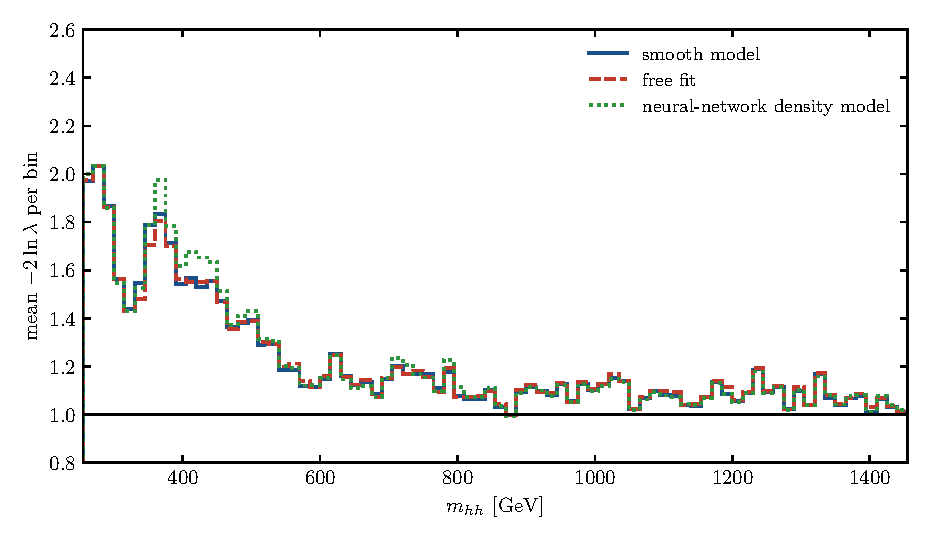
\includegraphics[width=0.72\textwidth]{fig_B_accuracy.pdf}
\caption{Mean $-2\ln\lambda$ per bin on the test spectra as a function of $m_{hh}$, for the smooth model, the free fit and the
neural-network density model.}
\label{fig:B:accuracy}
\end{figure}

\paragraph{Calibration and the model-error term.} The network has no fit uncertainty of its own; its pulls are computed with the
Poisson noise and a model-error term of the form~(\ref{eq:A:syst}), with $A_{ik}$ from the network and $\varepsilon(m)$
determined on the held-out bins exactly as in appendix~\ref{app:A:syst}. Its $\varepsilon(m)$ agrees with the smooth model's
from threshold to about 1~TeV (0.070\% and 0.077\% at 262~GeV; 0.275\% and 0.279\% at 600~GeV), and with either the pulls are
calibrated at every degree of cancellation (table~\ref{tab:B:calibration}, figure~\ref{fig:B:calibration}). Two models built
in entirely different ways need the same model-error term: it is a property of the POWHEG spectra, not of either model. Above
1~TeV, where the bins hold about 20 events, the network's $\varepsilon$ is lower (2.9\% against 3.7\% at 1.45~TeV).

\begin{figure}[!htbp]
\centering
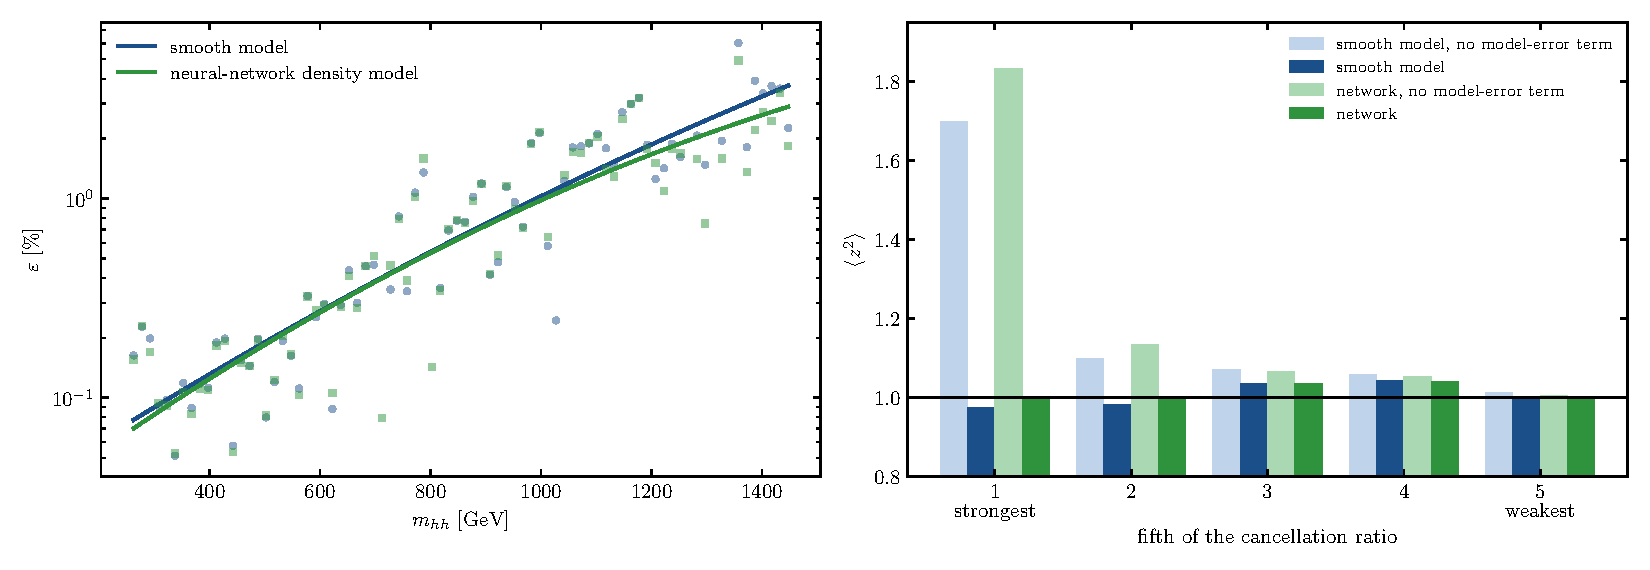
\includegraphics[width=\textwidth]{fig_B_calibration.pdf}
\caption{Left: the model-error coefficient $\varepsilon(m_{hh})$ of the two models, per bin (points) and in its smooth form
(lines). Right: $\langle z^2\rangle$ of the pulls by fifth of the cancellation ratio, with and without the model-error term.}
\label{fig:B:calibration}
\end{figure}

\paragraph{The density.} The two models can be compared at any $m_{hh}$, not only through bin integrals. On a 0.5~GeV grid from
255 to 1455~GeV, at the 1,000 test points, the network's $d\sigma/dm_{hh}$ differs from the smooth model's by a median of 0.31\%
(0.19\% below 555~GeV), and equally at the bin centres (0.30\%) and between them (0.32\%); 90\% of the differences lie within the
smooth model's total $\pm1\sigma$ (fit uncertainty and model-error term) and 98\% within $\pm2\sigma$.
Just above threshold the agreement is weaker. Below 350~GeV the median difference is 0.41\%, comparable to the smooth
model's total uncertainty there (a median 0.54\% of the density), and 85\% of the differences lie within $\pm2\sigma$.
There the differences oscillate on the scale of the bin width while the bin integrals agree (figure~\ref{fig:B:density}):
the data determine the bin integrals but not the shape of the density on scales finer than a bin, and each model fills
in that shape according to its own smoothness. On such scales just above threshold, the difference between the two
models is a better measure of the uncertainty of the density than the smooth model's band. The coefficient functions agree with those of the smooth model to 0.04--0.5\%
of their size for $a_1$--$a_{15}$ and 1.0--1.3\% for $a_{20}$--$a_{23}$; the poorly determined $a_{16}$--$a_{19}$ differ by 2--8\%, well
within the smooth model's own uncertainties for them (figure~\ref{fig:B:coefficients}).

\begin{figure}[!htbp]
\centering
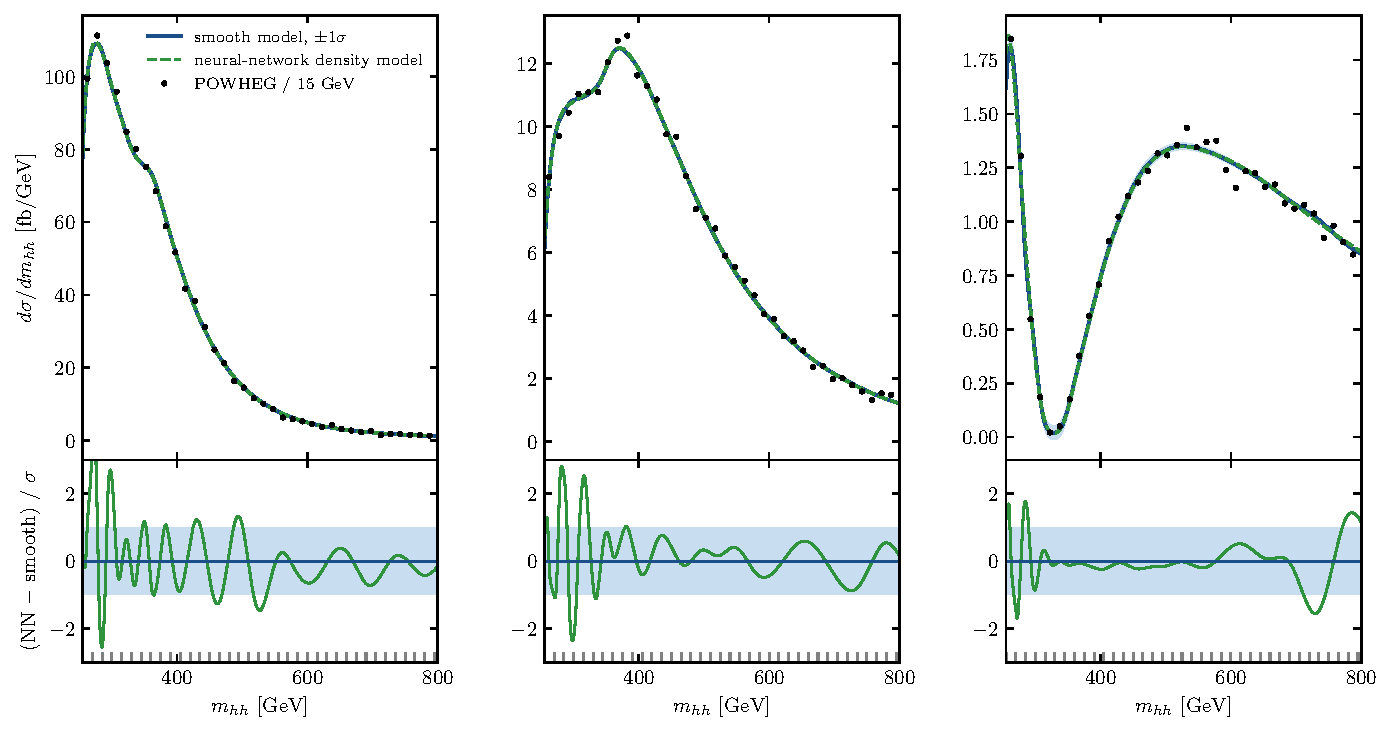
\includegraphics[width=\textwidth]{fig_B_density.pdf}
\caption{The density $d\sigma/dm_{hh}$ of the two models below 800~GeV for three test spectra, with POWHEG divided by the bin width.
Lower panels: the difference between the models in units of the smooth model's total uncertainty; the ticks mark the bin
edges.}
\label{fig:B:density}
\end{figure}

\paragraph{Inside a bin.} Trained on the 30~GeV bins of appendix~\ref{app:A:validation} with the same procedure, the
network predicts the split of each 30~GeV bin into its two 15~GeV halves at least as well as the smooth model
(figure~\ref{fig:B:merged}): the $\chi^2$ per pair is 1.06 on average between 360 and 555~GeV (smooth model 1.17), and
4.7, 2.7 and 3.3 in the first three pairs (smooth model 11, 3.9 and 4.1). Trained on the 15~GeV bins, the two models
predict the split equally well.

\begin{figure}[!htbp]
\centering
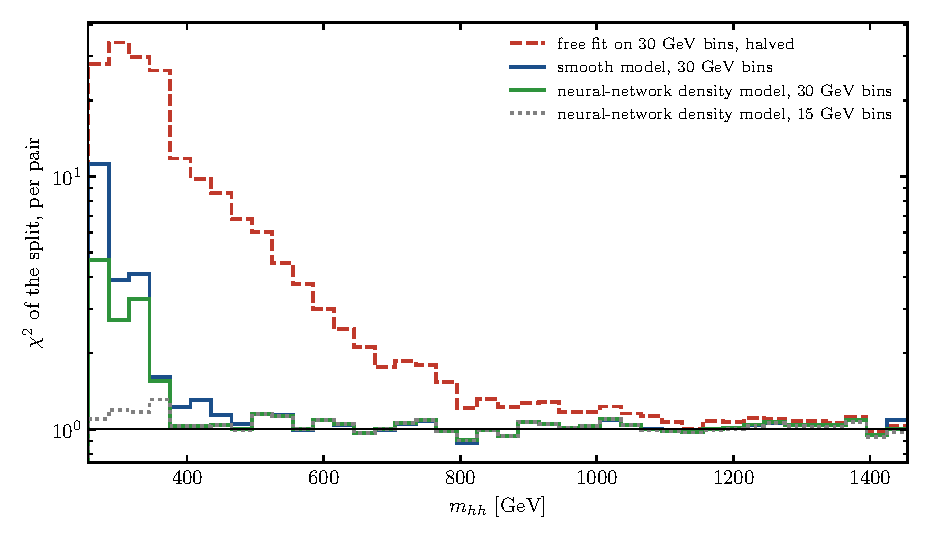
\includegraphics[width=0.72\textwidth]{fig_B_merged.pdf}
\caption{The merged-bin test of figure~\ref{fig:A:merged}, with the neural-network density model trained on the 30~GeV bins.}
\label{fig:B:merged}
\end{figure}

\paragraph{Below the fitted range.} Summed over the test spectra, the network predicts the unused bin 240--255~GeV 7\% high, as the
smooth model does.

\paragraph{Limitations.} The network is a single fit: it has no fit uncertainty of its own, which an ensemble of networks trained
from different random initial values would provide. Below 555~GeV its accuracy is slightly below that of the smooth model. For these
reasons the smooth model is the model of this paper, and the network an independent check of it.

\begin{figure}[p]
\centering
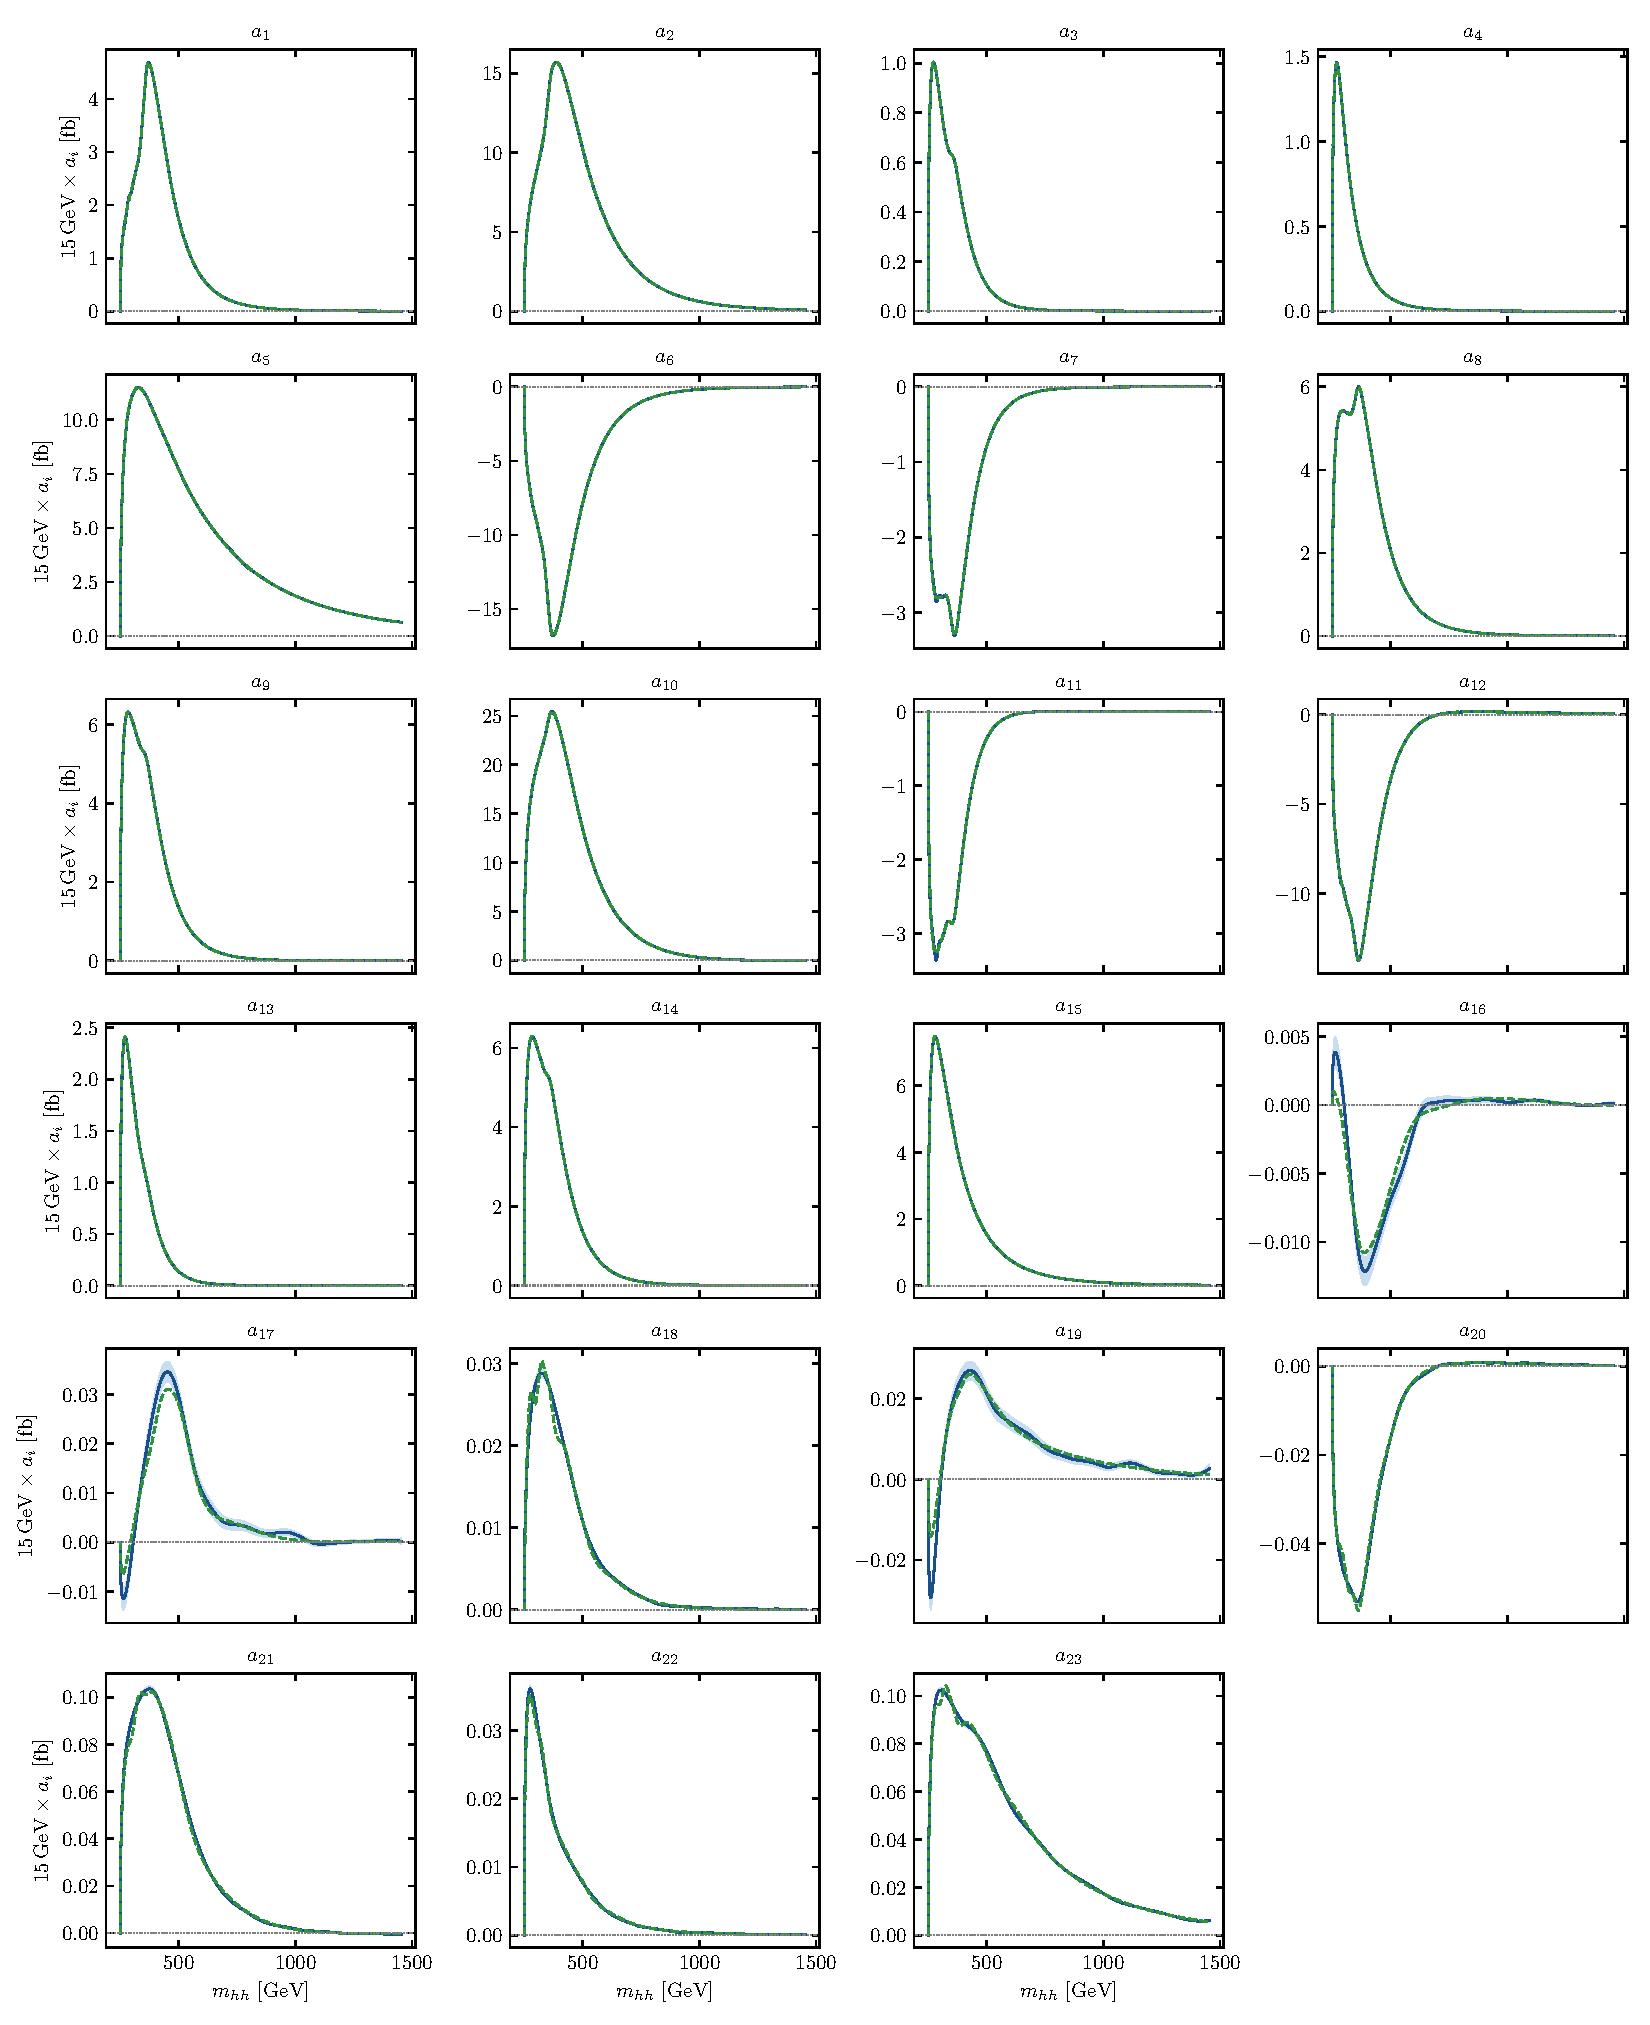
\includegraphics[width=\textwidth]{fig_B_coefficients.pdf}
\caption{The 23 coefficient functions of the neural-network density model (dashed) over those of the smooth model with their
$\pm1\sigma$ bands, as in figure~\ref{fig:A:coefficients}.}
\label{fig:B:coefficients}
\end{figure}
